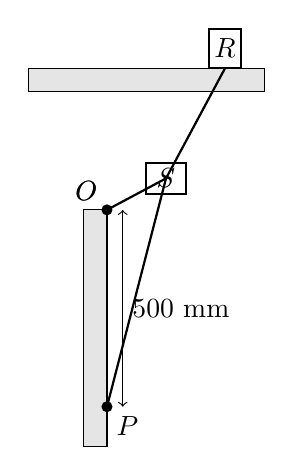
\begin{tikzpicture}
    % Draw the vertical wall
    \draw[fill=gray!20] (-0.3,-3) rectangle (0,0);

    % Draw the horizontal support for block R
    \draw[fill=gray!20] (-1,1.5) rectangle (2,1.8);

    % Draw point P
    \fill (0,-2.5) circle (2pt) node[below right] {$P$};

    % Draw point O (pivot)
    \fill (0,0) circle (2pt) node[above left] {$O$};

    % Draw the vertical dimension line for 500 mm
    \draw[<->] (0.2,0) -- (0.2,-2.5) node[midway, right] {500 mm};

    % Draw block R as a rectangle above
    \draw[thick] (1.3,1.8) rectangle (1.7,2.3) node[midway] {$R$};

    % Draw block S as a rectangle
    \draw[thick] (0.5,0.2) rectangle (1.0,0.6) node[midway]{ $S$ };

    % Draw the connections between points without passing through blocks
    \draw[thick] (1.5,1.8) -- (0.75,0.4); % Connecting R to S
    \draw[thick] (0.75,0.4) -- (0,0);     % Connecting S to O
    \draw[thick] (0,0) -- (0,-2.5);       % Connecting O to P
    \draw[thick] (0,-2.5) -- (0.75,0.4);  % Connecting P to S directly

    % Label point O
    \node[above left] at (0,0) {$O$};
    % Label point S only once, placing it effectively
    \node[above right] at (0.75,0.4) { };

\end{tikzpicture}


